
\section{Molecular Imaging Methods}	% You can also have slides prior to the first section or work entirely without sections.

\begin{frame}[c]{Cryo-Electron Microscopy (Cryo-EM)}
    \begin{itemize}
        \item Enables observation of molecules in near atomic resolution.
        \item Major motivation for Thesis.
        \item During freezing, molecules rotate randomly.
        \item Frozen molecules are fragile, electron microscope needs to work with low power.
        \item Observations can be reconstructed to 3D model.
    \end{itemize}

    \begin{tcolorbox}[colback=red!5!white,hide=<-1>, alert=<2>, colframe=red!75!black]
        Only single particle cryo-EM is considered.
    \end{tcolorbox}

\end{frame}

\begin{frame}[c]{Cryo-EM}
    \begin{figure}
        \captionsetup[subfigure]{justification=centering}
        \centering
        \hfill
        \begin{subfigure}[t]{0.35\textwidth}
            \vskip 0pt
            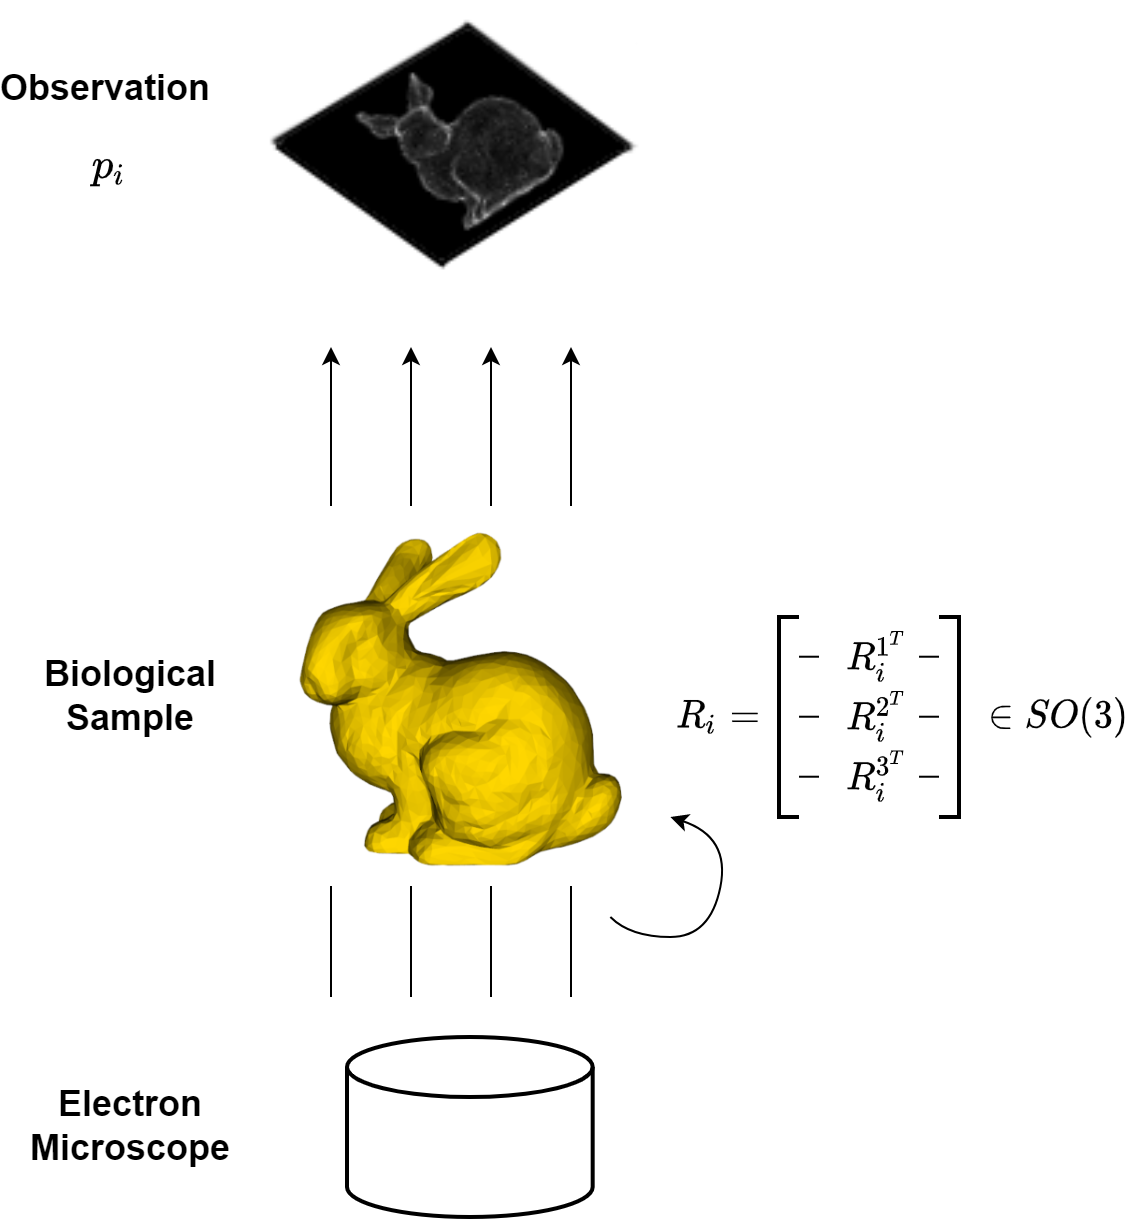
\includegraphics[width=\textwidth]{CryoObservation.drawio.png}
        \end{subfigure}\hfill
        \only<2>{
            \begin{subfigure}[t]{0.4\textwidth}
                \vskip 0pt
                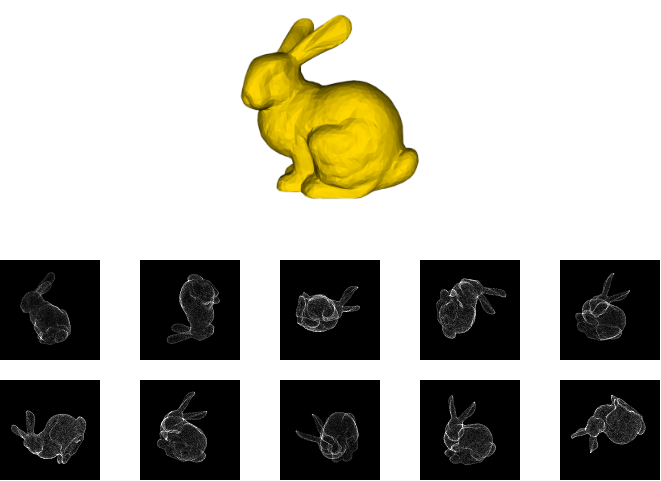
\includegraphics[width=\textwidth]{Cryo-EM_reconstruction.drawio.png}
            \end{subfigure}\hfill
        }
        \caption{Cryo-EM overview}
    \end{figure}

\end{frame}

\begin{frame}[c]{Cryo-EM challenges}
    \begin{columns}[c]
        \column{.45\textwidth}
        
        \begin{itemize}
            \item High-noise level 
            \item Unknown rotation during freezing
            \item (Structural variety of observations)
        \end{itemize}

        % \begin{tcolorbox}[colback=red!5!white,hide=<-1>, alert=<2>,colframe=red!75!black]
        %     Master Thesis domain of interest is to high-noise regime (cryo-EM).
        %     Goal is to introduce a denoise method for cryo-EM 2D projections.
        % \end{tcolorbox}

        \column{.55\textwidth}
        \begin{figure}
            \centering
            \begin{subfigure}[t]{0.5\textwidth}
                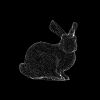
\includegraphics[width=\textwidth]{bunny_872.png}
                \caption{Clean micrograph}
            \end{subfigure}\hfill                
            \begin{subfigure}[t]{0.5\textwidth}
                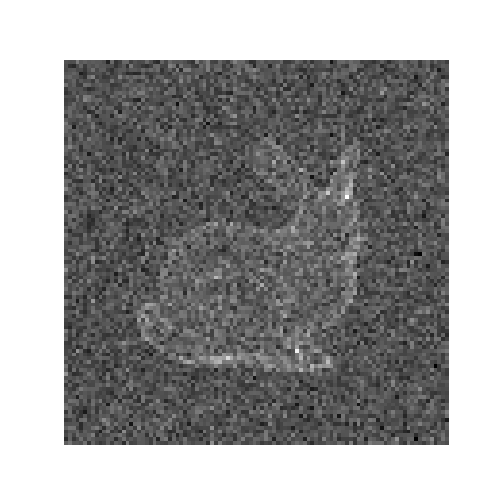
\includegraphics[width=\textwidth]{bunny_872_noisy.png}
                \caption{Noisy micrograph}
            \end{subfigure}\hfill                
        \end{figure}

    \end{columns}

    %\footnotetext[1]{https://www.ebi.ac.uk/emdb/EMD-32177}
\end{frame}

%\begin{frame}
%    \begin{definition}[Cryo-EM observation]
%        $$ y_i[j,k] = \Pi_z (\; Rot(\;x; \theta_i))_{j,k} + \eta_i[j,k], \text{ with } 1 \leq i \leq N \text{ and } 1 \leq j,k \leq M,$$
%    \end{definition}
%    \begin{itemize}
%        \item $y_i[] \in \tilde{\Omega}, x \in L^2(\Omega)$ with $\Omega \subset \mathbb{R}^3 $ and $\tilde{\Omega} \subset \mathbb{R}^2 $
%        \item $M$ observation dimension
%        \item $\Pi_z : L^2(\Omega) \to L^2(\tilde{\Omega})$ projection operator
%        \item $Rot : L^2(\Omega) \to L^2(\Omega),$ is rotation operator
%        \item $Rot(x, \theta_i) = \left((x_1,x_2,x_3) \mapsto x( x_1R^1_{\theta_i}, x_2R^2_{\theta_i}, x_3R^3_{\theta_i})\right)$
%        \begin{itemize}
%            \item $\theta_i = [\theta_i^{(1)}, \theta_i^{(2)}, \theta_i^{(3)} ] $, with $\theta_i^{(1)}, \theta_i^{(2)}, \theta_i^{(3)} \in \mathbb{R}$
%            \item $R_{\theta_i} =  [R^1_{\theta_i}, R^2_{\theta_i}, R^3_{\theta_i}] \in SO(3)$ is the 3D rotation matrix 
%        \end{itemize}
%    \end{itemize}
%\end{frame}


\begin{frame}[c]{Computed Tomography (CT)}
    \begin{columns}[c]
        \column{.55\textwidth}
            \begin{itemize}
                \item Related to cryo-EM
                \item Can be seen as a simpler version in 2D
                \item Good to start with towards a cryo-EM algorithm
            \end{itemize}
        
        \column{.45\textwidth}
        \begin{figure}
            \centering
            \begin{subfigure}[t]{0.45\textwidth}
                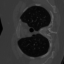
\includegraphics[width=\textwidth]{ct_im_2}
                \caption{Biological sampel}
            \end{subfigure}\hfill                
            \begin{subfigure}[t]{0.51\textwidth}
                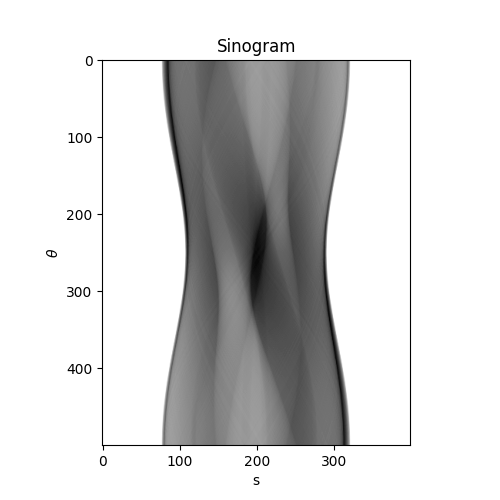
\includegraphics[width=\textwidth]{phantom_sino}
                \caption{clean Sinogram}
            \end{subfigure}\hfill          
        \end{figure}

        
    \end{columns}
\end{frame}


\begin{frame}{Observation}

    \begin{block}{Observation}
        \only<1>{
            \begin{equation}
                \begin{aligned}
                    y &= p + \eta \\
                \end{aligned}
            \end{equation}
        }
        
        \only<2->{
            \begin{equation}
                \begin{aligned}
                    y &= p + \eta \\
                    y_i &=  A(x, \theta_i) \\
                    y_i[j] &= p_i[j] + \eta_i[j] & \text{ with } 1 \leq i \leq N, 1 \leq j \leq M  \\
                \end{aligned}
            \end{equation}
        }

    \end{block}

    \only<1-2>{

    
        \begin{columns}[T]
        \column{.5\textwidth}

        
        \begin{itemize}
            \item<1-> $y$: noisy observation
            \item<1-> $p$: noiseless observation
            \item<1-> $\eta$: noise, assumed  $\eta_i \sim \mathcal{N}(0,\sigma^2)$
            \item<2-> $\theta_i$: observation angle
        \end{itemize}
            
        \column{.5\textwidth}

        \begin{itemize}
            \item<2-> $A: L^2(\Omega) \to \mathbb{R}^M, x \mapsto A(x; \theta_i)$: \\a non-linear operator 
            \item<2-> $N$: number of observations
            \item<2-> $M$: observation dimension
        \end{itemize}

        \end{columns}
    }
    
    \only<3>{
        \begin{tcolorbox}[colback=red!5!white,colframe=red!75!black]
            $SNR_y$ is used to define the level of noise of observation.    
        \end{tcolorbox}
    }
    
        
\end{frame}

\begin{frame}{Observation - Computed Tomography }

    \begin{figure}
    \centering
    \begin{subfigure}{0.4\textwidth}
        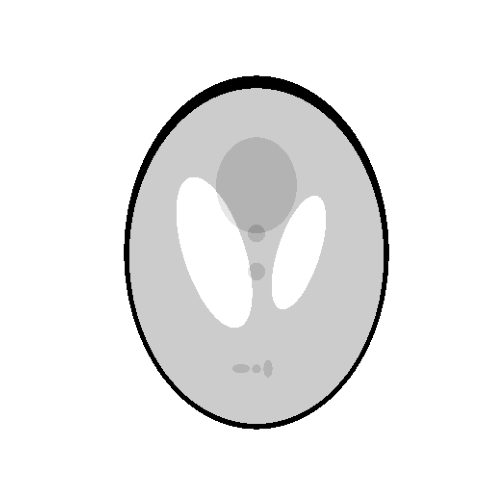
\includegraphics[width=\textwidth]{phantom.png}
        \caption{Biological Sample}
    \end{subfigure}
    \begin{subfigure}{0.4\textwidth}
        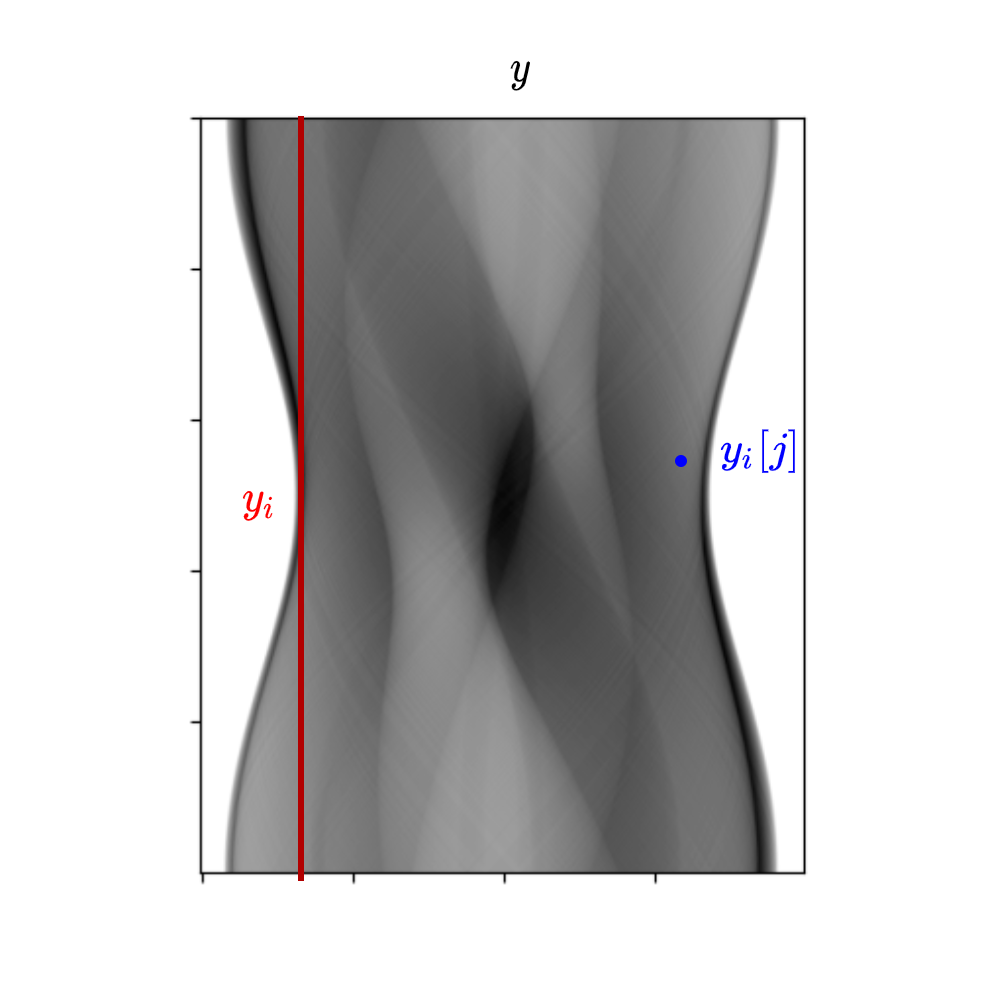
\includegraphics[width=\textwidth]{sino_yi.drawio.png}
        \caption{CT Observation - sinogram}
    \end{subfigure}
\end{figure}

\end{frame}


\begin{frame}{Observation - Cryo-EM }

    \begin{figure}
        \centering
        \begin{subfigure}[t]{0.3\textwidth}
            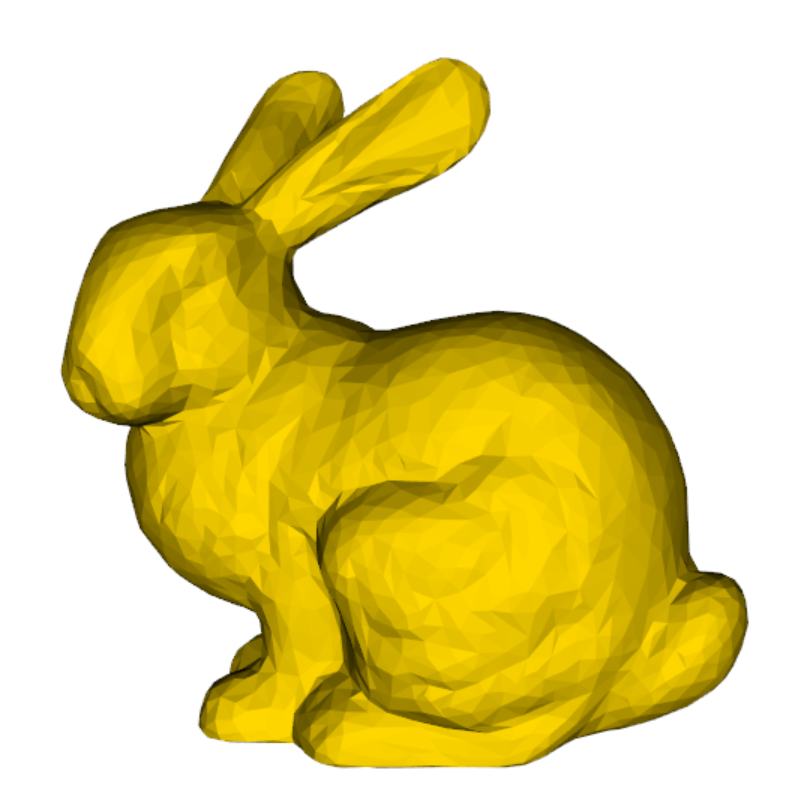
\includegraphics[width=\textwidth]{bunny.PNG}
            \caption{Biological Sample}
        \end{subfigure}
        \begin{subfigure}[t]{0.65\textwidth}
            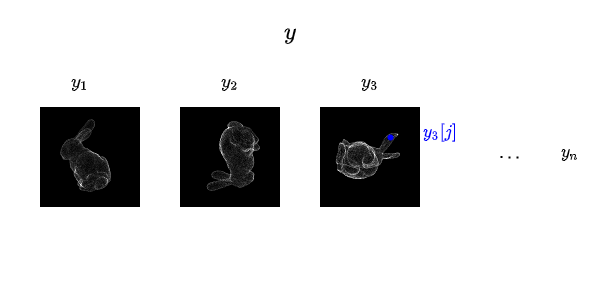
\includegraphics[width=\textwidth]{micrograph_yi.drawio.png}
            \caption{Cryo-EM Observation - micrographs}
        \end{subfigure}
    \end{figure}

\end{frame}



\begin{frame}{Reconstruction}

    \begin{block}{Reconstruction}
        \begin{equation}
            \begin{aligned}
                \textit{Recon} : & \mathbb{R}^{M \times N} \to \mathbb{R}^{M \times M} & y \mapsto Recon(y; \theta)
            \end{aligned}
        \end{equation}
    \end{block}

\end{frame}

\begin{frame}{Reconstruction -  Computed Tomography}
    \begin{columns}
        \column{.45\textwidth}
        
        \begin{itemize}
            \item Filter Backprojection (FBP)
            \begin{itemize}
                \item Can be considered historical approach
                \item Enables reconstruction for moderate noise.
            \end{itemize}
            \item<2> Neural Network Approaches
            \begin{itemize}
                \item Today state-of-the art
                \item Using result of FBP and further denoise.
                \item U-Net \cite{unet-tomography}.
            \end{itemize}
        \end{itemize}

        \column{.55\textwidth}
        \begin{figure}
            \centering
            \begin{subfigure}[t]{0.45\textwidth}
                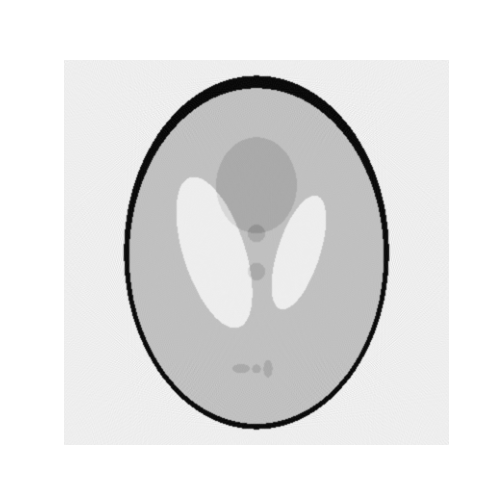
\includegraphics[width=\textwidth]{fbp_phantom_clean.png}
                \caption{Reconstruction clean: \\
                    $Recon(p, \theta) \approx x$}
            \end{subfigure}
            \begin{subfigure}[t]{0.45\textwidth}
                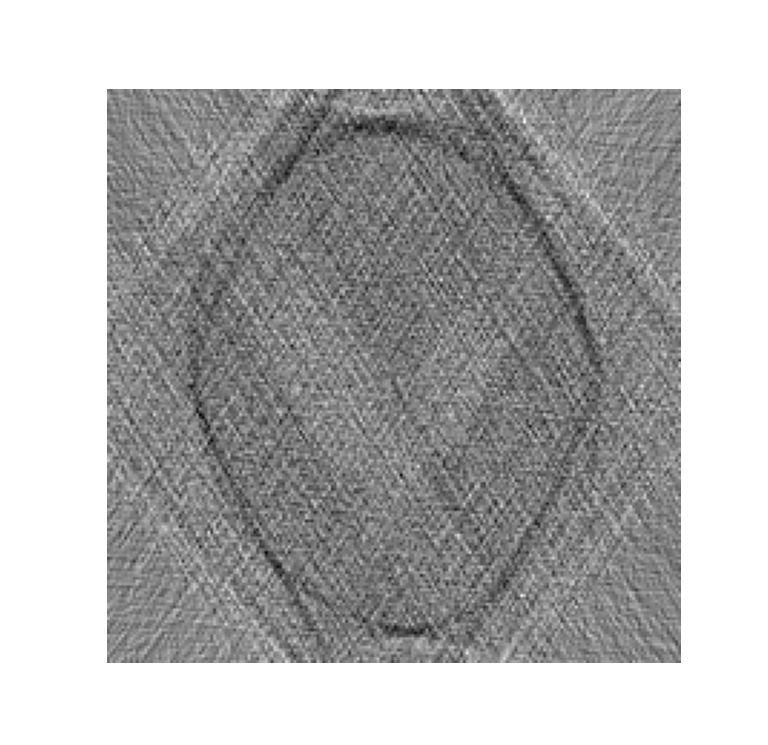
\includegraphics[width=\textwidth]{fbp_phantom_snr_0.png}
                \caption{Reconstruction noisy: \\
                    $Recon(p, \theta) \not\approx x$}
            \end{subfigure}
        \end{figure}
    \end{columns}

\end{frame}



\begin{frame}{Problem and Goal}
    
    \begin{block}{Problem}
        $p$ not observable directly only $y$ is observable.
    \end{block}

    \begin{block}{Goal}
        $$ denoiser:   y_i = (p_i + \eta) \mapsto p_i^* \approx p_i $$
        $$ \textit{Recon} \left( denoiser(y; \theta) \right) \approx x $$
    \end{block}

\end{frame}


